\index{interpolation}
\chapter{Interpolation \& Extrapolation}
\newthought{Reconstructing Functions from Scattered Data}


% ==============================================================================================
% INTRODUCTION BLOCK

\section{The Why}
\index{interpolation!motivation}

\newthought{In the previous chapters,} we assumed we could evaluate $f(x)$ wherever we wanted.
But in practice, data comes as discrete samples:
\begin{equation}
    \{(x_0, y_0), (x_1, y_1), \ldots, (x_n, y_n)\}
\end{equation}

\newthought{The interpolation problem:} Find a function $p(x)$ such that $p(x_i) = y_i$ for all $i$.

\newthought{Why this matters:}
\begin{itemize}
    \item Sensor data comes at discrete time points
    \item Images are pixel grids, not continuous functions
    \item Training data is a finite sample from a distribution
\end{itemize}

\marginnote{\newthought{The universal approximation theorem} says neural networks can approximate any continuous function. But what does ``approximate'' mean? Interpolation theory gives precise answers.}

\newthought{In machine learning and artificial intelligence:}
\begin{itemize}
    \item \textbf{Neural networks are function approximators:} They interpolate/approximate training data
    \item \textbf{Overfitting $\leftrightarrow$ Runge phenomenon:} Perfect fit on training points, wild behavior elsewhere
    \item \textbf{Data augmentation:} Creating new samples by interpolating between real ones (Mixup)
    \item \textbf{Distribution shift:} Extrapolation to out-of-distribution inputs fails badly
\end{itemize}

\newthought{Key lesson:} The mathematics of interpolation explains why overfitting happens and why extrapolation is dangerous.



\newpage
\subsection{Hands On Experience}
\index{interpolation!hands-on}

\newthought{Consider fitting} a polynomial through $(0, 1)$, $(1, 0)$, $(2, 1)$.

\vspace{1em}
\textbf{Linear interpolation} (using only first two points):
\begin{equation}
    p_1(x) = 1 - x
\end{equation}

Check: $p_1(0) = 1$ \checkmark, $p_1(1) = 0$ \checkmark, $p_1(2) = -1$ \ding{55}

\vspace{1em}
\textbf{Quadratic interpolation} (using all three points):

We need $p_2(x) = a + bx + cx^2$ satisfying:
\begin{align*}
    p_2(0) &= a = 1 \\
    p_2(1) &= a + b + c = 0 \\
    p_2(2) &= a + 2b + 4c = 1
\end{align*}

Solving: $a = 1$, $b = -2$, $c = 1$, so $p_2(x) = 1 - 2x + x^2 = (x-1)^2$.

\marginnote{\newthought{Notice:} More points $\Rightarrow$ higher degree polynomial. Three points determine a unique parabola.}

Check: $p_2(0) = 1$ \checkmark, $p_2(1) = 0$ \checkmark, $p_2(2) = 1$ \checkmark

\begin{figure}[h]
    \centering
    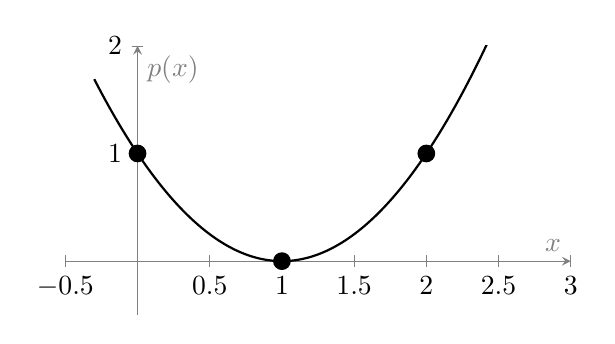
\begin{tikzpicture}
        \begin{axis}[
            width=8cm,
            height=5cm,
            axis x line=middle,
            axis y line=middle,
            xlabel={$x$},
            ylabel={$p(x)$},
            xmin=-0.5, xmax=3,
            ymin=-0.5, ymax=2,
            tick style={gray},
            label style={gray},
            axis line style={gray},
        ]
        % Quadratic
        \addplot[black, thick, smooth, domain=-0.3:2.5, samples=50] {(x-1)^2};
        % Points
        \addplot[black, only marks, mark=*, mark size=3pt] coordinates {(0, 1) (1, 0) (2, 1)};
        \end{axis}
    \end{tikzpicture}
    \caption{Quadratic interpolation through three points gives the parabola $(x-1)^2$.}
    \label{fig:quadratic_interp}
\end{figure}


\vspace{2.5em}
\newthought{The Learning Objectives} of this chapter aim at providing you with the abilities to:
\begin{itemize}
    \item Derive and apply Lagrange interpolation
    \item Understand and recognize Runge's phenomenon
    \item Explain why high-degree polynomial interpolation is dangerous
    \item Connect interpolation theory to overfitting in machine learning
    \item Distinguish interpolation from extrapolation and understand the risks
\end{itemize}




% ==============================================================================================
% MAIN THEORY BLOCK

\newpage
\section{The Interpolation Problem}
\index{interpolation!problem statement}

\newthought{Given:} Data points $(x_0, y_0), (x_1, y_1), \ldots, (x_n, y_n)$ with distinct $x_i$.

\newthought{Find:} A function $p(x)$ such that $p(x_i) = y_i$ for all $i = 0, 1, \ldots, n$.

\newthought{Questions:}
\begin{itemize}
    \item Does such a function exist?
    \item Is it unique?
    \item How should $p(x)$ behave between the data points?
\end{itemize}

\newthought{Polynomial interpolation:} Seek $p(x) = a_0 + a_1 x + \cdots + a_n x^n$ of degree $\leq n$.

\begin{theorem}[Existence and Uniqueness]
Given $n+1$ points with distinct $x$-coordinates, there exists a unique polynomial of degree $\leq n$ passing through all points.
\end{theorem}

\marginnote{\newthought{Proof idea:} The system of equations $p(x_i) = y_i$ gives $n+1$ equations in $n+1$ unknowns (the coefficients). The Vandermonde matrix is invertible when all $x_i$ are distinct.}




\newpage
\section{Lagrange Interpolation}
\index{Lagrange interpolation}

\newthought{Idea:} Construct basis polynomials $L_i(x)$ such that:
\begin{equation}
    L_i(x_j) = \begin{cases} 1 & \text{if } i = j \\ 0 & \text{if } i \neq j \end{cases}
\end{equation}

Then the interpolating polynomial is simply:
\begin{equation}
    p(x) = \sum_{i=0}^{n} y_i \cdot L_i(x)
\end{equation}

\newthought{Construction of $L_i(x)$:}

$L_i(x)$ must be zero at all $x_j$ except $x_i$. This suggests:
\begin{equation}
    L_i(x) = \frac{\prod_{j \neq i} (x - x_j)}{\prod_{j \neq i} (x_i - x_j)}
\end{equation}

The numerator is zero at each $x_j$ (for $j \neq i$), and the denominator ensures $L_i(x_i) = 1$.

\newthought{The Lagrange interpolation formula:}
\begin{equation}
    \boxed{p(x) = \sum_{i=0}^{n} y_i \prod_{j \neq i} \frac{x - x_j}{x_i - x_j}}
\end{equation}

\newthought{Example:} Interpolate through $(0, 1)$, $(1, 0)$, $(2, 1)$.

\begin{align*}
    L_0(x) &= \frac{(x-1)(x-2)}{(0-1)(0-2)} \\
    &= \frac{(x-1)(x-2)}{2} \\[6pt]
    L_1(x) &= \frac{(x-0)(x-2)}{(1-0)(1-2)} \\
    &= \frac{x(x-2)}{-1} \\
    &= -x(x-2) \\[6pt]
    L_2(x) &= \frac{(x-0)(x-1)}{(2-0)(2-1)} \\
    &= \frac{x(x-1)}{2}
\end{align*}

\begin{align*}
    p(x) &= 1 \cdot L_0(x) + 0 \cdot L_1(x) + 1 \cdot L_2(x) \\
    &= \frac{(x-1)(x-2)}{2} + \frac{x(x-1)}{2} \\
    &= \frac{(x-1)[(x-2) + x]}{2} \\
    &= \frac{(x-1)(2x-2)}{2} \\
    &= (x-1)^2
\end{align*}

This matches our earlier result!

\marginnote{\newthought{Complexity:} Computing $p(x)$ at one point costs $O(n^2)$ operations. There are more efficient algorithms (Neville's, barycentric) with $O(n)$ per evaluation.}




\newpage
\section{Runge's Phenomenon}
\index{Runge's phenomenon}

\newthought{A cautionary tale:} Higher-degree polynomials are not always better.

\newthought{Runge's function:}
\begin{equation}
    f(x) = \frac{1}{1 + 25x^2}
\end{equation}

on the interval $[-1, 1]$.

\begin{figure}[h]
    \centering
    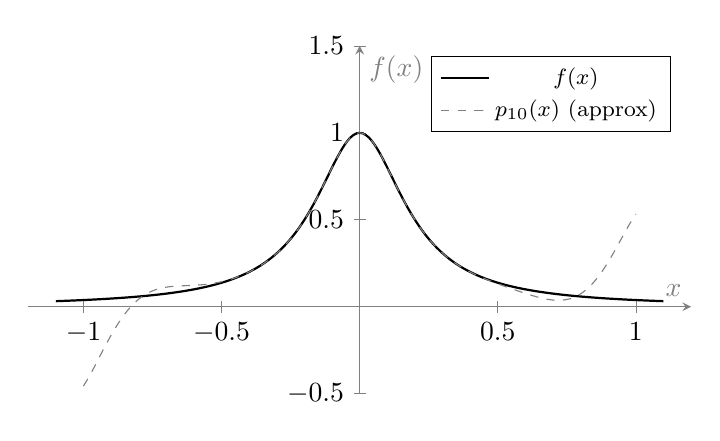
\begin{tikzpicture}
        \begin{axis}[
            width=10cm,
            height=6cm,
            axis x line=middle,
            axis y line=middle,
            xlabel={$x$},
            ylabel={$f(x)$},
            xmin=-1.2, xmax=1.2,
            ymin=-0.5, ymax=1.5,
            tick style={gray},
            label style={gray},
            axis line style={gray},
            legend pos=north east,
            legend style={font=\footnotesize},
        ]
        % True function
        \addplot[black, thick, smooth, domain=-1.1:1.1, samples=100] {1/(1 + 25*x^2)};
        \addlegendentry{$f(x)$}
        % Approximate degree 10 polynomial behavior (oscillates at edges)
        \addplot[gray, dashed, smooth, domain=-1:1, samples=100]
            {1/(1 + 25*x^2) + 0.5*sin(deg(8*x))*x^6};
        \addlegendentry{$p_{10}(x)$ (approx)}
        \end{axis}
    \end{tikzpicture}
    \caption{Runge's phenomenon: the polynomial interpolant oscillates wildly near the boundaries, despite passing through all data points.}
    \label{fig:runge}
\end{figure}

\newthought{What happens:}
\begin{itemize}
    \item $n = 5$ points: polynomial looks reasonable
    \item $n = 11$ points: oscillations appear at edges
    \item $n = 21$ points: even worse oscillations!
\end{itemize}

\marginnote{\newthought{Maximum error:}
\begin{itemize}
    \item $n = 5$: max error $\approx 0.4$
    \item $n = 11$: max error $\approx 2$
    \item $n = 21$: max error $\approx 60$
\end{itemize}
More points make it \textbf{worse}!}

\newthought{Why this happens:} The polynomial must pass through all points, but between points (especially near boundaries), it can oscillate wildly to ``connect the dots.''

\newthought{Mathematically:} The error bound for polynomial interpolation includes a factor $\prod_{i=0}^n (x - x_i)$, which can be large for equally spaced points.




\newpage
\section{Connection to Overfitting}
\index{overfitting}

\newthought{Runge's phenomenon is overfitting!}

\begin{table*}[ht]
\centering
\begin{tabular}{p{0.35\textwidth}p{0.43\textwidth}}
\toprule
\textbf{Interpolation} & \textbf{Machine Learning} \\
\midrule
Data points $(x_i, y_i)$ & Training examples \\
Polynomial degree $n$ & Model complexity / \# parameters \\
Perfect fit $p(x_i) = y_i$ & Zero training error \\
Wild oscillations & Poor generalization \\
Runge phenomenon & Overfitting \\
\bottomrule
\end{tabular}
\vspace{2em}
\caption{Runge's phenomenon in interpolation directly parallels overfitting in machine learning.}
\label{tab:interpolation_ml_analogy}
\end{table*}

\marginnote{\newthought{The bias-variance tradeoff:}
\begin{itemize}
    \item Low degree: high bias (underfitting)
    \item High degree: high variance (overfitting)
    \item Optimal: balance between the two
\end{itemize}}

\newthought{Key insight:} A model that perfectly fits training data (interpolates) may perform terribly on new data, especially if:
\begin{itemize}
    \item The model is too flexible (high degree / many parameters)
    \item Data points are noisy
    \item We're asked to extrapolate beyond the training range
\end{itemize}

\newthought{Solutions in ML mirror solutions in interpolation:}
\begin{itemize}
    \item \textbf{Regularization:} Penalize complexity (like using lower-degree polynomials)
    \item \textbf{Splines:} Piecewise polynomials instead of one global polynomial
    \item \textbf{Early stopping:} Don't fit the training data perfectly
    \item \textbf{Dropout, weight decay:} Reduce effective model capacity
\end{itemize}




\newpage
\section{Extrapolation}
\index{extrapolation}

\newthought{Interpolation:} Estimate $f(x)$ for $x$ between data points.

\newthought{Extrapolation:} Estimate $f(x)$ for $x$ \emph{outside} the data range.

\begin{figure}[h]
    \centering
    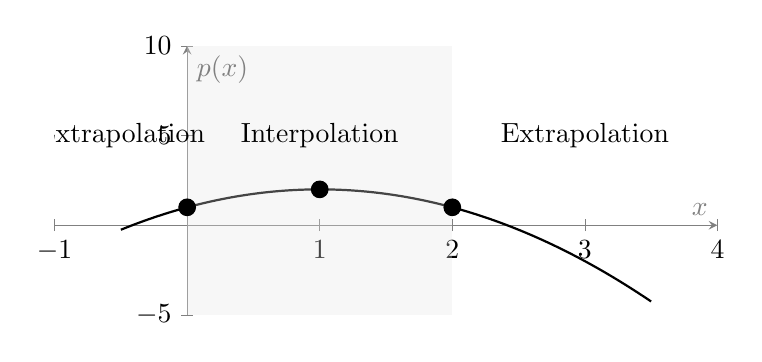
\begin{tikzpicture}
        \begin{axis}[
            width=10cm,
            height=5cm,
            axis x line=middle,
            axis y line=middle,
            xlabel={$x$},
            ylabel={$p(x)$},
            xmin=-1, xmax=4,
            ymin=-5, ymax=10,
            tick style={gray},
            label style={gray},
            axis line style={gray},
        ]
        % Quadratic through (0,1), (1,2), (2,1)
        \addplot[black, thick, smooth, domain=-0.5:3.5, samples=50] {1 + 2*x - x^2};
        % Data range
        \addplot[fill=gray!20, draw=none, opacity=0.3] coordinates {(0, -5) (0, 10) (2, 10) (2, -5)};
        % Points
        \addplot[black, only marks, mark=*, mark size=3pt] coordinates {(0, 1) (1, 2) (2, 1)};
        % Extrapolation region labels
        \node at (axis cs:-0.5, 5) {Extrapolation};
        \node at (axis cs:3, 5) {Extrapolation};
        \node at (axis cs:1, 5) {Interpolation};
        \end{axis}
    \end{tikzpicture}
    \caption{Inside the data range (shaded), interpolation is reasonable. Outside, extrapolation quickly diverges.}
    \label{fig:extrapolation}
\end{figure}

\newthought{Why extrapolation is dangerous:}
\begin{itemize}
    \item Polynomials grow unboundedly: $x^n \to \pm\infty$ as $x \to \pm\infty$
    \item No data to constrain the function outside the range
    \item Small changes in data can cause large extrapolation changes
\end{itemize}

\marginnote{\newthought{In ML, extrapolation = distribution shift.} A model trained on ImageNet performs poorly on sketches, a spam classifier trained on 2020 emails fails on 2025 emails.}

\newthought{In deep learning:}
\begin{itemize}
    \item \textbf{Distribution shift:} Test data differs from training data
    \item \textbf{Out-of-distribution detection:} Recognize when input is outside training range
    \item \textbf{Domain adaptation:} Adjust model for new domains
\end{itemize}

\newthought{Rule of thumb:} Never trust a model's predictions far from its training data.




% ==============================================================================================
% STUDENT ACTIVATION BLOCK

\newpage
\section{Examples \& Exercises}
\index{interpolation!exercises}

\marginnote{\newthought{Code} can be found at \url{https://github.com/Quillstacks/lecturecode_numericalmethods.git}.}

\newthought{Exercise 1: Lagrange by hand.} Find the Lagrange interpolating polynomial through $(−1, 3)$, $(0, 1)$, $(1, 3)$.

\textit{Setup:}
\begin{align*}
    L_0(x) &= \frac{(x-0)(x-1)}{(-1-0)(-1-1)} = \frac{x(x-1)}{2} \\
    L_1(x) &= \frac{(x+1)(x-1)}{(0+1)(0-1)} = -(x^2-1) = 1 - x^2 \\
    L_2(x) &= \frac{(x+1)(x-0)}{(1+1)(1-0)} = \frac{x(x+1)}{2}
\end{align*}

Compute $p(x) = 3 L_0(x) + 1 L_1(x) + 3 L_2(x)$ and simplify.


\vspace{2em}
\newthought{Exercise 2: Runge's phenomenon.} For $f(x) = 1/(1 + 25x^2)$ on $[-1, 1]$:
\begin{enumerate}
    \item Sample at $n+1$ equally spaced points for $n = 5, 10, 15, 20$
    \item Compute Lagrange interpolant at each $n$
    \item Plot $f(x)$ and $p_n(x)$ for each case
    \item Compute $\max_{x \in [-1,1]} |f(x) - p_n(x)|$
\end{enumerate}

Observe how error \emph{increases} with $n$!


\vspace{2em}
\newthought{Exercise 3: Extrapolation danger.} Fit a cubic through $(0, 1)$, $(1, 2)$, $(2, 2)$, $(3, 0)$.
\begin{enumerate}
    \item Compute the interpolating polynomial
    \item Evaluate at $x = -1, 4, 5$
    \item Are these extrapolated values reasonable?
\end{enumerate}


\vspace{2em}
\newthought{Exercise 4: Overfitting analogy.} Consider noisy data:
\begin{equation}
    y_i = \sin(x_i) + \epsilon_i, \quad \epsilon_i \sim \mathcal{N}(0, 0.1)
\end{equation}

sampled at 10 points in $[0, 2\pi]$.
\begin{enumerate}
    \item Fit polynomial of degree 3, 5, 9
    \item Compare training error vs. test error (on new points)
    \item Which degree generalizes best?
\end{enumerate}




\newpage
\section{Self-Reflection and Recap}
\index{interpolation!recap}

\newthought{Self-Reflection} Questions to guide your understanding:
\begin{itemize}
    \item How is Runge's phenomenon like overfitting?
    \item Why does early stopping in DL help with generalization?
    \item What's the difference between interpolation and regression?
    \item Why are neural networks not plagued by Runge's phenomenon? (Hint: regularization, architecture)
    \item What happens when you ask ChatGPT about events after its training cutoff?
\end{itemize}

\newthought{Recap} of Key Concepts:
\begin{itemize}
    \item \textbf{Lagrange interpolation:} Unique polynomial of degree $\leq n$ through $n+1$ points.
    \item \textbf{Runge's phenomenon:} High-degree polynomials oscillate wildly, especially at boundaries.
    \item \textbf{Overfitting:} Perfect training fit $\neq$ good generalization.
    \item \textbf{Extrapolation:} Predicting outside training range is unreliable and dangerous.
\end{itemize}


\marginnote{\newthought{Teaser.} Fitting one global polynomial through all points causes oscillations. What if we fit \textbf{many small polynomials} and connect them smoothly? This is the idea behind splines.}

\newthought{From global to local.} The problems with polynomial interpolation stem from using one global polynomial. In the next chapter, we'll see how \emph{splines}---piecewise polynomials with smoothness constraints---avoid Runge's phenomenon while maintaining accuracy.



%%%%%%%%%%%%%%%%%%%%%%%%%%%%%%%%%%%%%%%%%%%%%%%%%%%%%%%%%%%%%%%%%%%%%%%%%%%%%%
